\begin{frame}{Une prise de conscience nécessaire 1/2}
\begin{block}{Évolution des architectures applicatives}
\begin{itemize}
\item Applications clients-serveurs légers \pause
\item Recours aux technologies Web 2.0 (PHP, Javascript, Bootstrap, etc) \pause
\item Recours aux API (B2B Network Manager par exemple) \pause
\item Utilisation de technologies de conteneurisation telles que Docker \pause
\end{itemize}
\end{block}
\begin{block}{Évolution des méthodes de développement}
\begin{itemize}
\item Mise en retrait de la DTI \pause
\item Cycle de développement et de déploiement plus courts (cf ASAP, itérativité, etc) \pause
\item Diminution des RH mais contraintes maintenues  
\end{itemize}
\end{block}
\end{frame}

\begin{frame}{Une prise de conscience nécessaire 2/2}
\begin{block}{Evolution des méthodes de gestion de projet}
\begin{itemize}
\item Eviter l'effet tunnel en livrant plus souvent \pause
\item Déployer en continu \pause
\item Automatiser les tests (cf gitlab) \pause
\item Conserver une disponibilité maximum (sur panne et sur déploiement) par un retour arrière natif 
\end{itemize}
\end{block}
\end{frame}

\begin{frame}{Une dette technologique à combler}
\begin{block}{Un contrôle aérien qui a soif de modernité}
\begin{itemize}
    \item Décloisonnement des acteurs du TA (PC, FMP, CDS, Cie, NM, etc) \pause
    \item Numérisation et automatisation de l'information (\sout{téléphone}) \pause
    \item Une vitrine pour valoriser les compétences internes de la DSNA 
\end{itemize}
\end{block} 
 \begin{exampleblock}{Exemples d'applicatifs}
 WikiFF, 4Me, SALTO (sur SAVOIE), iStream, CCS (sur leur propre machines)
\end{exampleblock}
\begin{block}{Un existant peu optimal}
\begin{itemize}
\item Un bi-serveur par application (SIAM, EPEIRES, WikiFF) => N Serveurs physiques pour N/2 applicatifs (pertes de perfos) \pause
\item Une box Internet par applicatif (iSTREAM, SALTO, etc) \pause
\item Aucune mutualisation des services (3 applications sur SIAM-TECH, 3 serveurs MySQL) \pause
\item Chaque section doit se former sur des méthodes de travail similaires 
\end{itemize}
\end{block}
\end{frame}

%%%%%%%%%%%%%%%%%%%%%%%%%%%%%
% Les solutions
%%%%%%%%%%%%%%%%%%%%%%%%%%%%%
\begin{frame}{Une solution en deux temps}
\begin{block}{Deux salles, deux ambiances, un même plaisir}
\begin{itemize}
    \item Une solution nationale : Le réseau ATM2 
    \item Une solution locale : L'infrastructure SAVOIE
\end{itemize}
\end{block} 

\begin{alertblock}{Nécessité de différencier les deux}
\begin{itemize}
    \item Pas les mêmes matériels
    \item Pas les mêmes intervenants nationaux et locaux impliqués
\end{itemize}
\end{alertblock} 

\begin{alertblock}{Mais les deux ne sont pas bijectifs ! \#ClassePrepa}
\begin{itemize}
    \item SAVOIE nécessite forcément ATM2 a priori ... \footnote{vSphere ne sert pas à virtualiser des clients. On peut le faire si on veut mais ce n'est pas fait pour. Au premier ordre, si on utilise SAVOIE pour implémenter un système, on utilisera ATM2. Si on ne veut pas utiliser ATM2, on utilise une infra indépendante.}
    \item Mais on peut connecter des systèmes sur ATM2 sans utiliser l'infrastructure SAVOIE. 
\end{itemize}
\end{alertblock}
\end{frame}

\begin{frame}{Schéma très simplifié d'ATM2}
\begin{center}
    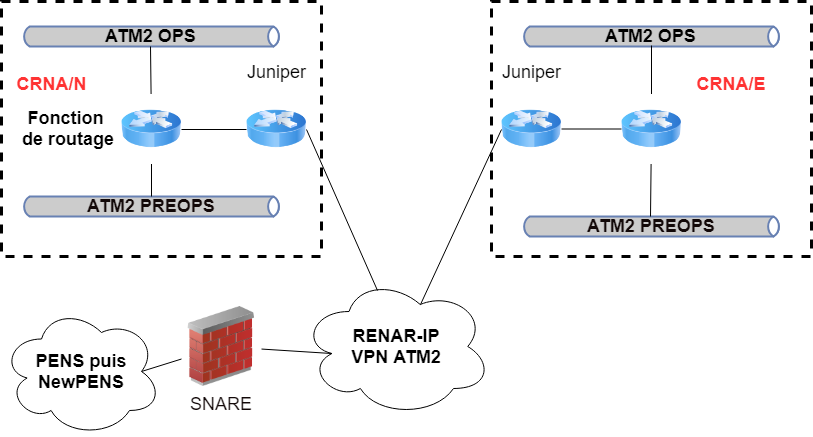
\includegraphics[width=330px]{Schemas/ATM2.png}
\end{center}
\end{frame}

\begin{frame}{Attention!}
\begin{block}{Ce cours n'évoque pas :}
\begin{itemize}
    \item ATM2 (du moins que de manière très superficielle) cf. cours de Mickael Papail
    \item les clients multiservices => La solution technique n'est pas encore définie. 
    \item la supervision réseaux et applicatifs => La solution technique n'est pas encore définie
\end{itemize}
\end{block}
\end{frame}

\begin{frame}{Objectif de la formation}
\begin{block}{Connaître un vocabulaire de base}
\begin{itemize}
\item ESX, ESXi, hôte, noeud, serveurs
\item VM, MV
\item Hyperviseur, VSphere
\item SAN, NAS, Datastore, LUN, Target 
\end{itemize}  
\end{block} 
\begin{block}{Etre à l'aise avec l'architecture SAVOIE}
\begin{itemize}
\item Connaître les grandes lignes du projet
\item Connaître les redondances de SAVOIE
\item Savoir se repérer dans vCenter
\item Savoir ce qu'un superviseur peut faire et ne doit pas faire
\item Etre capable d'avoir un discours clair et apaisé avec la salle
\end{itemize}  
\end{block} 
\end{frame}